\chapter{Perspectives et bilan}
\label{sec:Ending}
% Ce que nous avons fait
% Notre ressenti
% Y a t'il une place pour d'autres filtres de rehaussement ?
% Le rehaussement a t'il un futur ?

Dans les chapitres précédents, nous avons couvert l'ensemble de nos travaux sur l'analyse des filtres de rehaussement. Dans ce chapitre, nous proposons de discuter des perspectives futur du rehaussement. Nous commençons par discuter de la création de nouveaux filtres de rehaussement puis des possibilités d'utiliser le rehaussement pour la segmentation à base de deep learning. Nous abordons ensuite une application connexe, la segmentation des vaisseaux à partir de la seule annotation des bifurcations. Cette application, nous a menés à utiliser le rehaussement de vaisseaux pour tenter de localiser les bifurcations des vaisseaux dans un contexte à information limitée. Nous concluons ce chapitre par un bilan de nos travaux.
 
\section{Amélioration des filtres}

Après avoir analysé les filtres de rehaussement qui se sont démarqués ces vingt dernières années, on peut se demander s'il est encore nécessaire de créer de nouveaux filtres de rehaussement. Notre opinion est que les filtres existants couvrent déjà une part importante des besoins pour le rehaussement. Les mesures de tubularité des filtres comme Frangi, Jerman et Sato couvrent une large part des besoins en termes de modélisation des vaisseaux. Les propositions récentes en termes de filtres de rehaussement présentent des différences structurelles, par exemple en choisissant d'autres descripteurs de géométrie (ondelettes, moments de Zernike, etc.). Les derniers changements de paradigmes majeurs pour le rehaussement de vaisseaux ont été effectués avec la mesure de tubularité proposée par Jerman et la classification de l'orientation de chemins orientés de RORPO.

Dans le même ordre d'idée, nous n'avons pas étudié OOF de manière extensive, alors que le descripteur matriciel de flux permettrait d'associer à OOF des mesures de tubularité plus élaborées (Frangi, Sato, Jerman, etc.). Il est donc possible que ce couplage réduise les débordements de ce type de filtres par rapport à la taille réelle des vaisseaux.

Enfin, il est envisageable de proposer un filtre de rehaussement basé sur un apprentissage à base de deep learning. Cependant, il est difficile de cerner l'apport qu'aurait une telle méthode par rapport à des réseaux qui effectuent directement une segmentation. Par exemple un réseau Unet produit une carte de probabilité presque binaire puisque les vérités terrains sont des segmentations. Produire un réseau de neurones qui prédit un rehaussement demanderait une vérité terrain du rehaussement attendu. La vérité terrain de vaisseaux, en termes de carte de rehaussement, est encore plus difficile à définir qu'une segmentation manuelle. De plus, dans le cas où l'on utiliserait un filtre existant comme vérité terrain, le réseau issu de l'entrainement ne permettrait pas forcément de dépasser les limitations intrinsèques du filtre utilisé.

\section{Couplage avec la segmentation à base de deep learning}

Ces dernières années, le deep learning est devenu la technologie la plus explorée pour résoudre des tâches complexes de segmentation. En particulier,  on privilégie les méthodes de bout en bout (\textit{end-to-end}). Ces méthodes concentrent toute la chaîne de traitement dans un réseau de neurones. Celui-ci apprend de lui-même à élaborer un modèle, à extraire des caractéristiques et à segmenter un organe. Comme on a pu le voir précédemment, le rehaussement s'applique en amont des chaînes de traitement de la segmentation et il peut donc aussi s'appliquer en amont des réseaux de neurones. Le traitement des jeux de données en deep learning est particulièrement important, puisque dans ces systèmes, c'est le jeu de données qui va contrôler la capacité du réseau à se spécialiser sur un problème ou au contraire à le généraliser. Un jeu de données se doit donc d'être le plus représentatif du problème que l'on cherche à traiter.

Les filtres de rehaussement de vaisseaux peuvent faciliter cette représentativité, puisqu'ils permettent de mettre en valeur les vaisseaux tout en éliminant une partie des autres structures. On peut, de plus, utiliser différents filtres ou différentes paramétrisations, non nécessairement optimales, pour augmenter artificiellement nos données ou renforcer l'apprentissage de vaisseaux spécifiques.

Nous avons effectué un travail collaboratif \cite{Affane_2022_article_commun} dans le cadre du projet ANR avec Abir Affane et al. où nous avons fait l'expérience de tester plusieurs combinaisons de filtres de rehaussement (Jerman, Sato, RORPO et Zhang) et d'architectures de réseaux de neurones (U-net, Dense Net, MultiRes U-net). Les expériences ont été menées sur la base de l'Ircad avec les filtres optimisés dont les paramètres optimaux ont été trouvés par notre banc de test. Les résultats des expériences montrent que le rehaussement, en particulier le rehaussement homogène de Jerman, peut aider les réseaux à mieux segmenter les vaisseaux.

Ces observations ont été obtenues en entrainant les réseaux de deux manières : un premier entrainement où l'ensemble du volume contenant les vaisseaux était présenté au réseau et un second entrainement où seuls des blocs (coupes successives d'un volume de quelques voxels d'épaisseurs) étaient présentés au réseau (Fig. \ref{fig:full_vs_slab}). Dans le second cas, le nombre de vaisseaux, leur taille et la taille de leur voisinage était réduit. Le réseau de neurones a donc plus de difficultés à différencier les vaisseaux de leur contexte. L'ajout de filtres de rehaussement permet de compenser cette perte de contexte. Le réseau obtient ainsi des performances proches de l'entrainement avec des images entières.

\begin{figure}[!ht]
    \centering
    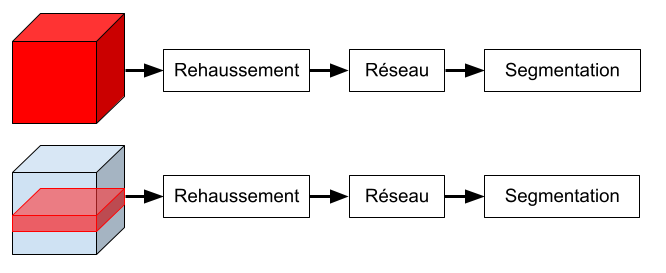
\includegraphics[height=6cm]{Images/full_vs_slab.png}
    \caption{Visualisation des deux types d'entrainement présentés dans \cite{Affane_2022_article_commun}. En haut, l'ensemble des volumes de la base de données est présenté au réseau après avoir été rehaussé. En bas, seul un bloc de quelques couches successives est utilisé. Le réseau doit donc apprendre à identifier les vaisseaux dans un contexte plus réduit. Les filtres de rehaussement, en particulier celui de Jerman, permettent de compenser la perte de performance due au contexte réduit.}
    \label{fig:full_vs_slab}
  \end{figure}

Survarachakan et al. \cite{Survarachakan2021_deep_vesselness} ont proposé des travaux similaires qui valident, eux aussi, l'utilisation des filtres de rehaussement afin d'améliorer la segmentation de réseaux de type U-net.

Les réseaux de neurones sont d'ailleurs connus pour avoir du mal à généraliser d'une modalité à une autre. En effet, l'apparence des vaisseaux peut changer selon les modalités ainsi que le contexte alentour. Les sorties des filtres de rehaussement ont aussi l'avantage d'être définis dans un domaine relativement homogène. On peut donc imaginer se servir des filtres de rehaussement pour unifier les modalités. On pourrait ainsi créer des jeux de données mixtes contenant des résultats de filtrages issus de modalités différentes et ainsi améliorer la généralisation des réseaux sur des images vasculaires, quelque soit leur modalité.

Une autre manière d'utiliser les filtres de rehaussement avec le deep learning est de considérer le résultat d'un filtrage comme un nouveau canal de l’image par analogie avec les images multi-spectrales. Ainsi, au lieu de remplacer les volumes présentés aux réseaux par des volumes filtrés, on concatène aux données initiales plusieurs filtrages. Un vaisseau est ainsi décrit par son aspect initial ainsi que par plusieurs types de rehaussements qui fournissent des données complémentaires. Lors de l'apprentissage, un réseau de neurones pourrait alors choisir la combinaison d'informations qui lui permettrait de segmenter au mieux les vaisseaux. \newV{ Ce type d'approches a déjà été employé pour la segmentation de tumeurs cérébrales en combinant des modalités IRM \cite{Wang2017_multiModal}.}

\section{Application connexe}

Vers la fin de nos travaux sur l'analyse de rehaussement, nous avons réalisé quelques expériences sur des sujets connexes au rehaussement. Ces expériences ont été guidées par une série d'observations que nous avons pu établir durant l'élaboration de nos travaux sur l'analyse du rehaussement des vaisseaux.

\subsection{Segmentation avec annotations réduites}

Nous avons indiqué à plusieurs reprises le long de ce manuscrit que la production d'annotationss est une tâche critique pour le développement de nouveaux algorithmes de segmentation de vaisseaux. Cependant, on ne peut pas demander à des médecins de consacrer des heures à l'annotation de volumes alors quelles pourraient être consacrées à prendre soin des patients. Le manque de personnel dans les hôpitaux ne semble pas aller dans le sens d'une amélioration prochaine de cette situation. À ces contraintes pratiques s'ajoute l'évolution des lois sur la gestion des données personnelles qui complexifie la collecte et la gestion des données. 

Ce contexte rend la constitution de larges bases de données plus difficile, données qui sont pourtant requises pour l'élaboration d'algorithmes basés sur l'apprentissage profond. Il y a donc une forme de contradiction entre l'évolution des solutions techniques et la réalité sur le terrain.  

En partant de ces observations, nous avons essayé de développer une méthode de segmentation qui réduit au maximum le temps d'annotation demandé aux médecins. En effet, la communauté est plus à même d'obtenir de larges bases de données annotées si le temps d'annotation d'un réseau vasculaire entier passe de 30 à 60 minutes à une dizaine de minutes. 

Pour atteindre cet objectif, il est nécessaire d'identifier des points remarquables des réseaux vasculaires. Les intersections entre plusieurs vaisseaux sont les seuls points qui sont à la fois critiques pour l'identification de la hiérarchie des vaisseaux et simples à identifier pour un annotateur. Ces bifurcations marquent en effet le début et la fin de chaque section tubulaire du réseau vasculaire. Elles peuvent donc ensuite servir comme points de départ et d'arrivée pour des algorithmes de tracking de vaisseaux.  De plus, si l'on demande au médecin de ne positionner qu'un seul point par bifurcation, le temps d'annotation s'en trouve drastiquement réduit. En comparaison, une segmentation des vaisseaux nécessite d'annoter l'ensemble des pixels des vaisseaux.
 
Une identification des vaisseaux à partir des bifurcations revient donc à :

\begin{itemize}
\item localiser les bifurcations ;
\item construire une hiérarchie entre les bifurcations ;
\item extraire le réseau vasculaire (ligne centrale ou segmentation).
\end{itemize}

\begin{figure}[!ht]
    \centering
    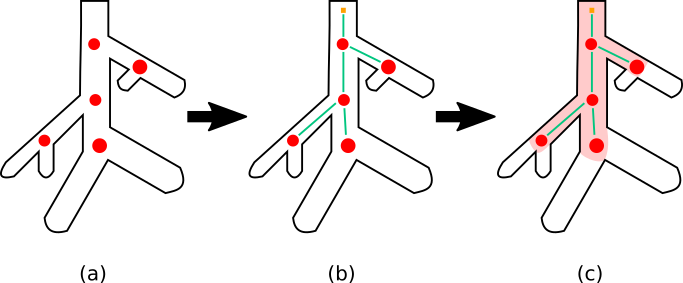
\includegraphics[width=\textwidth]{Images/thrifty_annotations.png}
    \caption{Segmentation avec annotations minimales. (a) Détection des bifurcations. (b) Construction d'un arbre hiérarchique par connexion entre les bifurcations. Cette connexion peut par exemple se faire grâce à une approche par chemins minimaux. (c) Segmentation du réseau vasculaire. On remarquera que les vaisseaux formant les extrémités du réseau vasculaire ne sont pas inclus dans cette méthode. Ils nécessitent donc un traitement particulier.}
    \label{fig:thrifty}
  \end{figure}

Une solution que nous avons envisagée pour l'extraction du réseau vasculaire a été de relier les bifurcations deux à deux grâce à une approche par chemins minimaux. L'optimisation du tracé de ce chemin peut alors reposer sur une carte de coût qui est le résultat d'un filtre de rehaussement de vaisseaux. Par exemple, pour trouver des chemins passant par le centre des vaisseaux, on peut choisir un filtre dont le rehaussement diminue près des bords. C'est le cas de filtres comme Frangi, Sato ou Jerman avec un $\tau$ élevé. Si l'on veut aller plus loin, il est aussi possible d'estimer le rayon des vaisseaux à partir de la ligne centrale ainsi obtenue (Fig. \ref{fig:thrifty}).

Le premier défi d'une telle méthode est donc la détection et la localisation des bifurcations. Nous présentons les différentes pistes que nous avons étudiées pour détecter ces structures et les problématiques auxquelles nous avons été confrontés. Ces travaux sont des ébauches dont nous illustrons quelques résultats préliminaires.

\subsubsection{Pistes de détection des bifurcations}

Le défi à relever est la détection et la localisation des bifurcations. En termes de modélisation, les bifurcations sont difficiles à définir. On considère d'habitude les bifurcations comme des zones en forme de blob, c'est-à-dire où le gradient s'éloigne du centre dans toutes les directions. Cette hypothèse est plus fragile lorsqu'elle est confrontée à la réalité des cas pratiques. Par exemple, si les vaisseaux composant la bifurcation ne font pas la même taille, la zone non tubulaire identifiant la bifurcation se trouve déportée sur les bords des vaisseaux et la géométrie se trouve plus aplatie que circulaire (Fig. \ref{fig:gradient_shift}). 

\begin{figure}[!ht]
    \centering
    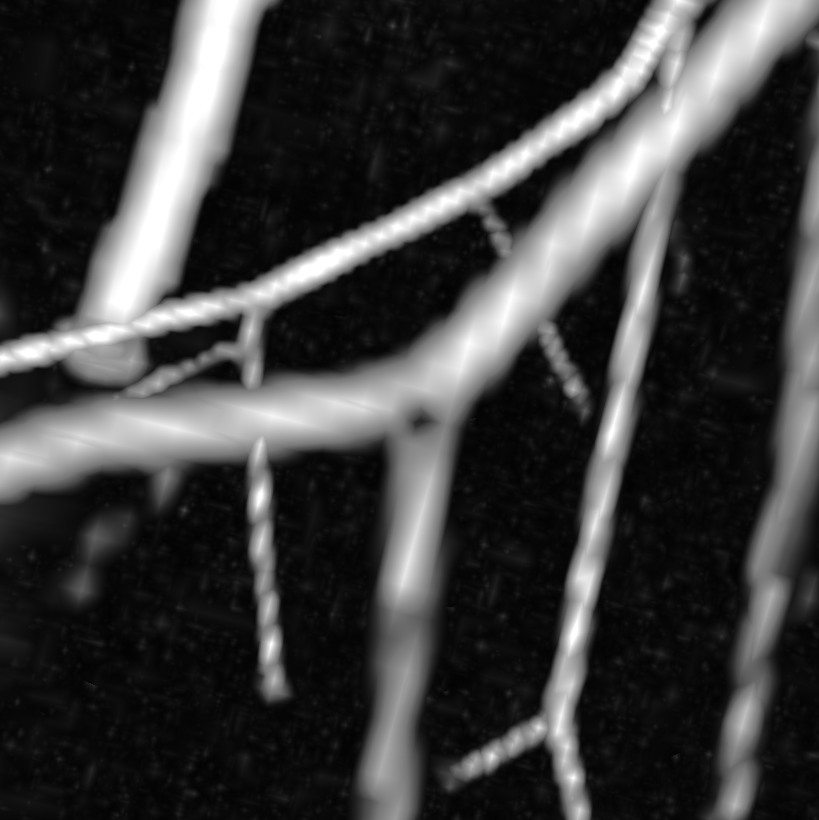
\includegraphics[height=5cm]{Images/Vascu_2_k_Sato.png}
    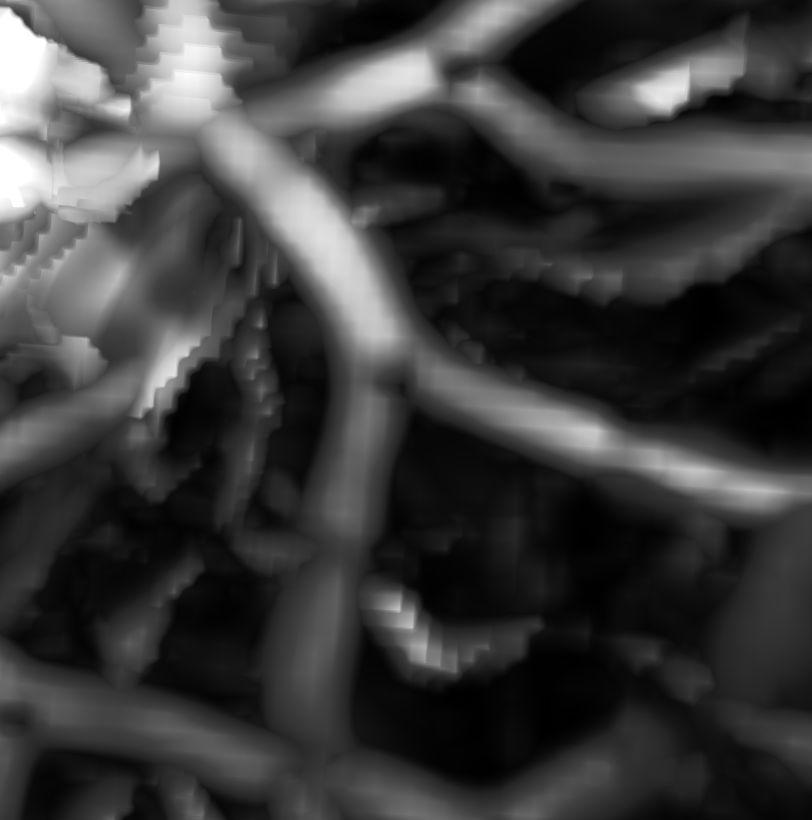
\includegraphics[height=5cm]{Images/Ircad_k_Sato.png}
    \caption{Filtre de Sato présentant une perte de signal marquée dans les zones non tubulaires, correspondant ici aux bifurcations. Lorsque les vaisseaux ne sont pas de même taille, la perte de signal ne se situe pas au centre, mais sur les bords du vaisseau principal.}
    \label{fig:gradient_shift}
\end{figure}

Par conséquent, la variabilité des bifurcations les rend difficile à modéliser par un filtre de rehaussement. Jerman et al. ont proposé un filtre de rehaussement pour les anévrismes qui ont, eux aussi, une structure en forme de blobs \cite{Jerman2015_blobness}. Cependant, le filtre de rehaussement proposé ne produit pas une réponse homogène. Cela atteste d'une géométrie réelle plus complexe. Les auteurs proposent d'ailleurs un système particulier de visualisation afin de compenser le manque de régularité de la réponse du filtre.

Nous avons testé ce filtre pour détecter les bifurcations sur des vaisseaux binaires du jeu de données VascuSynth. Les bifurcations y sont mal rehaussées, au contraire des pourtours des extrémités des vaisseaux, qui présentent une géométrie similaire aux anévrismes. Formuler une mesure d'appartenance à une bifurcation explicite est donc complexe à mettre en œuvre.  

\subsubsubsection{Composition de filtres de rehaussement}

Comme la détection explicite des bifurcations est difficile à réaliser, nous avons essayé de mettre en place une combinaison de filtres de rehaussement afin de les détecter de manière implicite. Au lieu de rechercher les bifurcations, nous recherchons les endroits non tubulaires. On inclut alors les variations de géométrie des bifurcations.

Nous avons en effet remarqué dans le chapitre précédent que pour certains filtres, une absence de signal distinct avait lieu au niveau des bifurcations (Fig. \ref{fig:gradient_shift}). En particulier, le filtre de Sato produit les pertes de signal aux bifurcations les plus marquées. On peut accentuer ce phénomène en paramétrant $\alpha_1$ avec des valeurs basses. 

On pourrait donc, a priori, utiliser la réponse inverse du rehaussement pour localiser les bifurcations. Toutefois, dans la réponse inverse, l'ensemble du fond serait rehaussé en même temps que les bifurcations. Afin de corriger ce problème, nous avons utilisé le filtre de Jerman avec une valeur de $\tau$ élevé afin de définir un masque qui différencie le fond des vaisseaux. Notre filtre $F(I)$ de détection de bifurcation s'exprime alors comme $F(I) = Jerman(I) - Sato(I)$ avec $I$ l'image d'entrée (Fig. \ref{fig:subtract_vesselness}). 

\begin{figure}[!ht]
    \centering
    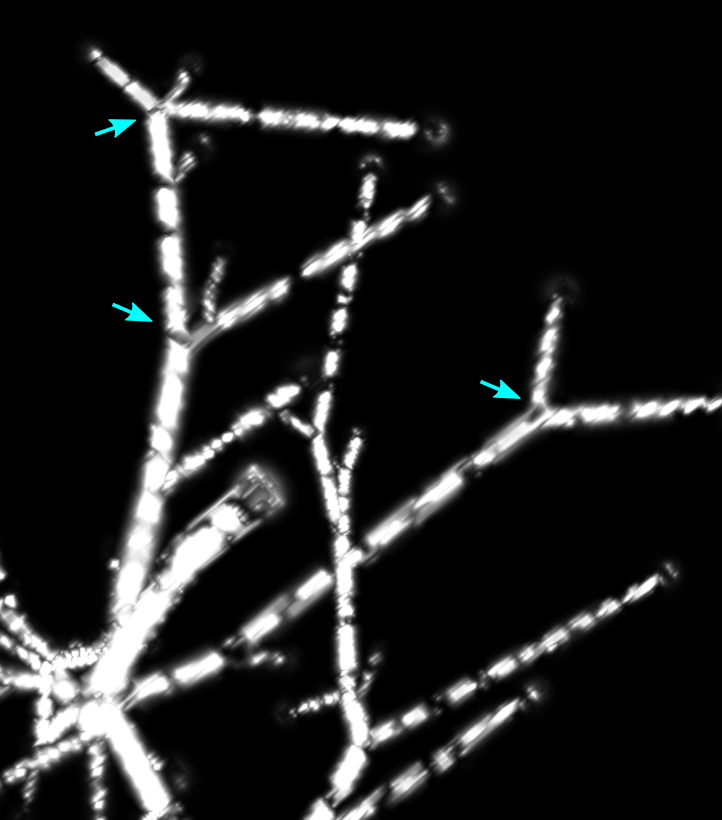
\includegraphics[height=4cm]{Images/SatoFilter_bif.png}
    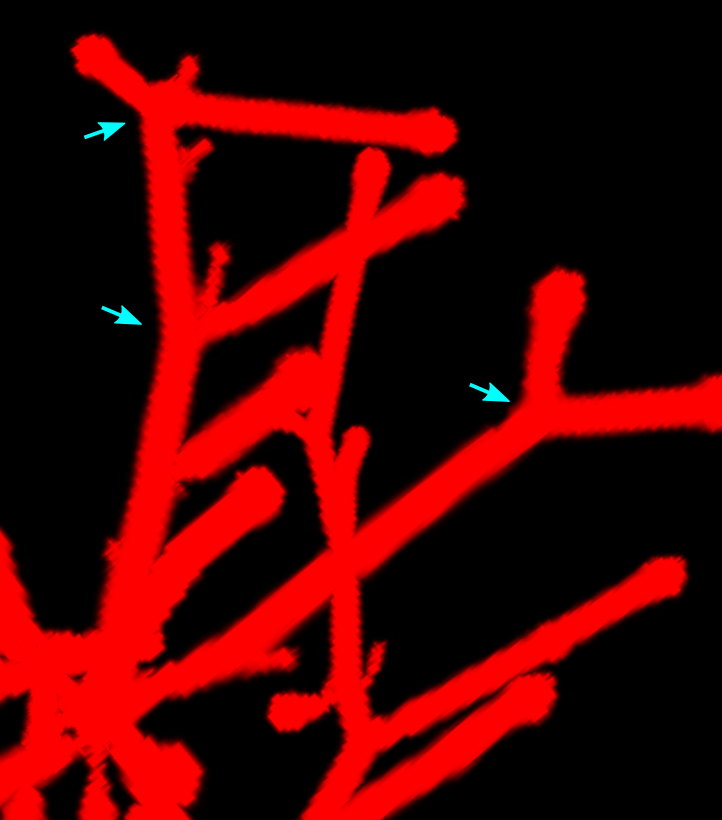
\includegraphics[height=4cm]{Images/JermanFilter_bif.png}
    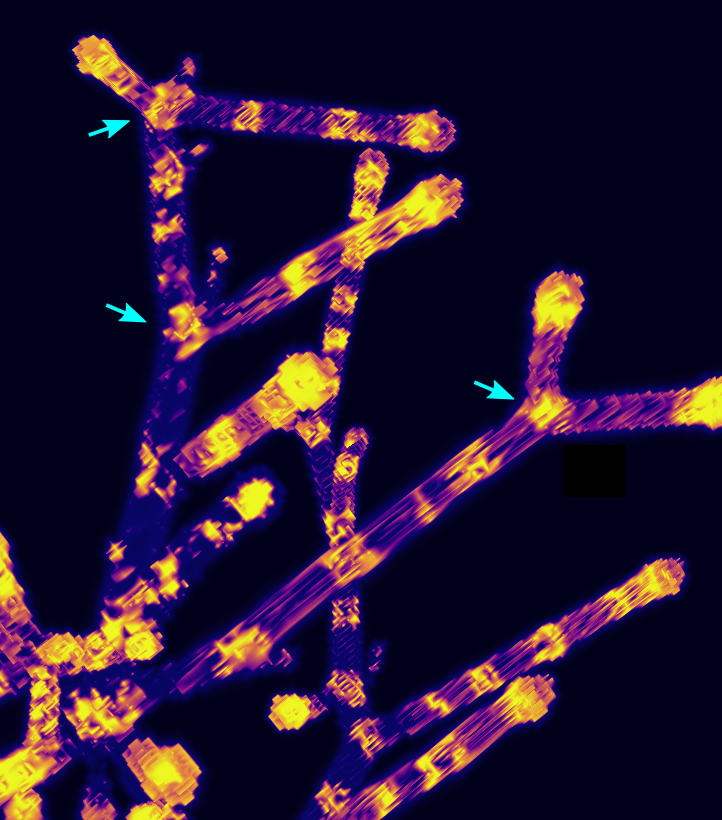
\includegraphics[height=4cm]{Images/subJermanSato_bif.png}
    \caption{Filtre de Sato (Blanc), Filtre de Jerman (Rouge), différence $\textrm{Jerman}-\textrm{Sato}$ (jaune). Bien que le signal du rehaussement soit plus fort sur les bifurcations, la visualisation en coupe suggère une exploitation difficile de cette méthode.}
    \label{fig:subtract_vesselness}
\end{figure}

Deux problèmes sont observables. Un résidu de signal est présent aux bifurcations, mais la délimitation de celui-ci est très variable. Il forme parfois des structures plates plutôt que sphériques. De plus, le filtre de Jerman estime le rayon des vaisseaux de manière plus large que le filtre de Sato. Le résultat forme une seule composante connexe formée d'une enveloppe externe et de cavités délimitées par des jonctions correspondant aux bifurcations. Dans ces structures, comparables à la structure d'un bambou, il reste difficile d'extraire les bifurcations (Fig. \ref{fig:combo_vesselness}).

\begin{figure}[!ht]
    \centering
    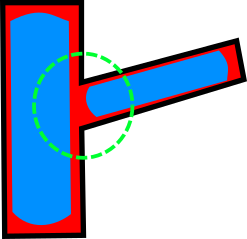
\includegraphics[height=6cm]{Images/combo_vesselness_2D.png}
    \caption{La différence (rouge) entre le filtre de Jerman et le filtre de Sato (bleu) produit une seule grande composante connexe. La réponse forte des vaisseaux est donc difficile à extraire de ce type de filtre composite.}
    \label{fig:combo_vesselness}
\end{figure}

\subsubsubsection{Détection par deep learning}

Face à la variabilité de la géométrie des bifurcations, nous nous sommes tournés vers des méthodes d'apprentissage à base de deep learning.

Nous avions à notre disposition des vérités terrain de segmentation voxéliques des bifurcations que nous avions construites dans le chapitre \chapBenchN{}. Nous nous sommes donc appuyés sur ces données pour essayer d'obtenir une segmentation voxélique des bifurcations sur le jeu de données VascuSynth, $\sigma=2$. Pour cela, nous avons choisi un réseau de segmentation, Unet, qui présentait de bons résultats pour la segmentation des vaisseaux (MCC $\approx 0.80$) sur ce jeu de données.

Cependant, lorsque les vérités terrains sont des segmentations des bifurcations, le réseau n'arrive pas à apprendre. Nous avons essayé de comprendre pourquoi en observant les résultats du réseau pour différentes étapes de l'entraînement (Fig. \ref{fig:seg_deep}). Nous avons alors remarqué que le réseau apprenait dans un premier temps à segmenter les vaisseaux avant de tenter d'apprendre les bifurcations. Toutefois, celui-ci ne parvient pas à différencier les bifurcations de tronçons quelconques du réseau vasculaire.

On peut néanmoins remarquer que Unet arrive à segmenter les bifurcations lorsqu'il est chargé de segmenter le réseau vasculaire entier, mais qu'il échoue lorsqu'il doit segmenter les bifurcations seules. La segmentation des bifurcations est donc probablement un sous-problème, plus complexe, de la segmentation des vaisseaux. 

Dans ce contexte, plusieurs hypothèses sont envisageable. Les vérités terrains des bifurcations qui incluent une partie des vaisseaux ne sont pas assez discriminantes pour différencier les bifurcations du reste des vaisseaux. Les bifurcations sont des structures trop rares pour être apprises correctement par le réseau de neurone.

\begin{figure}[!ht]
    \centering
    \begin{subfigure}{0.45\textwidth}
        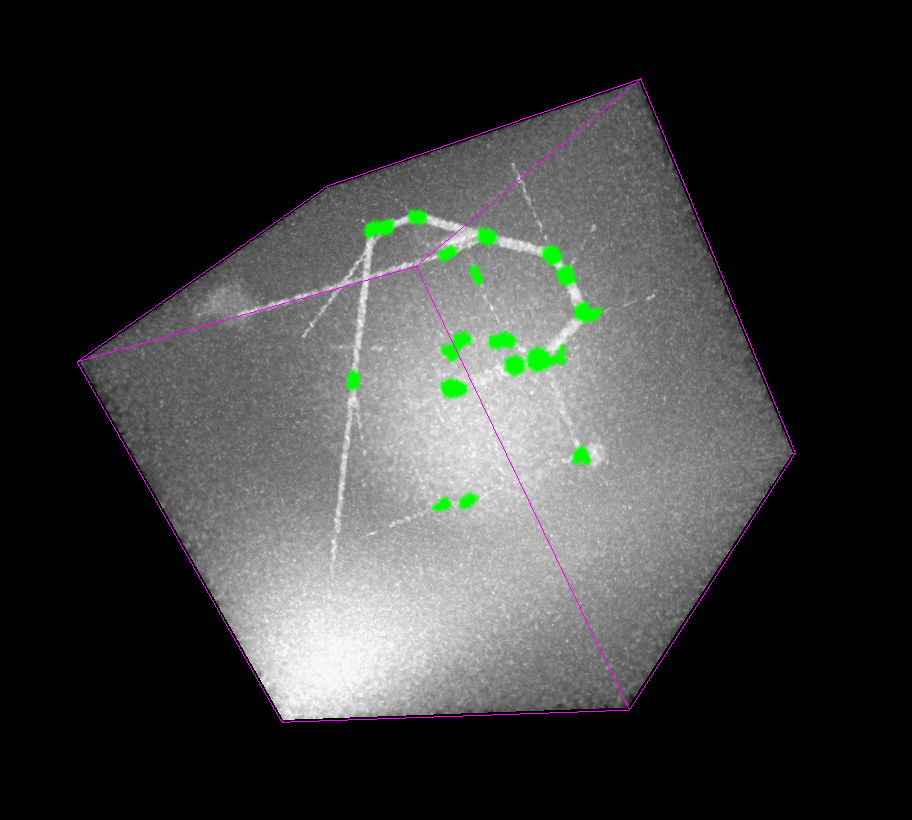
\includegraphics[width=\textwidth]{Images/exp_seg_gt.png}
        \caption{Vérité terrain}
    \end{subfigure}
    \begin{subfigure}{0.45\textwidth}
        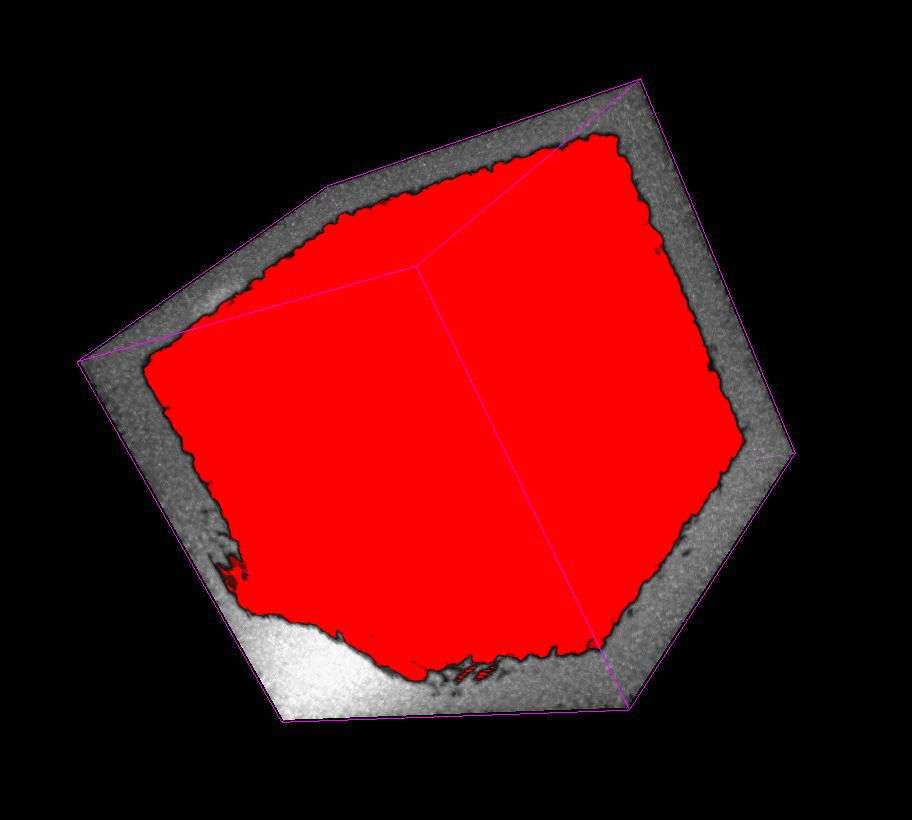
\includegraphics[width=\textwidth]{Images/exp_seg_40.png}
        \caption{Itération $40$}
    \end{subfigure}
    \begin{subfigure}{0.45\textwidth}
        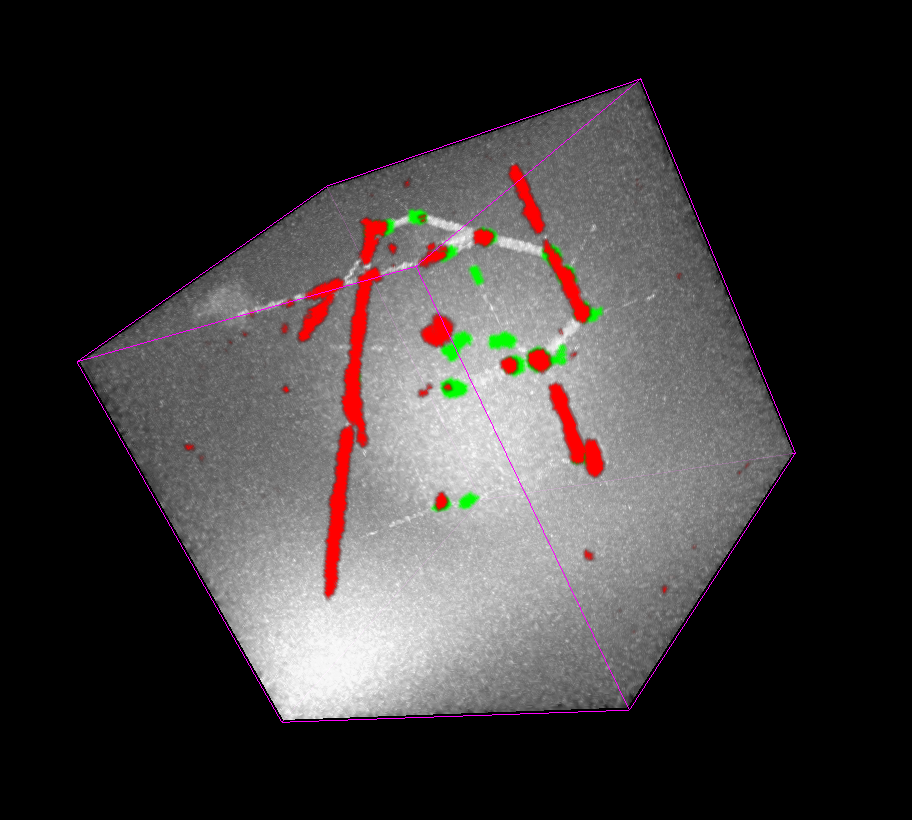
\includegraphics[width=\textwidth]{Images/exp_seg_100.png}
        \caption{Itération 100}
    \end{subfigure}
    \begin{subfigure}{0.45\textwidth}
        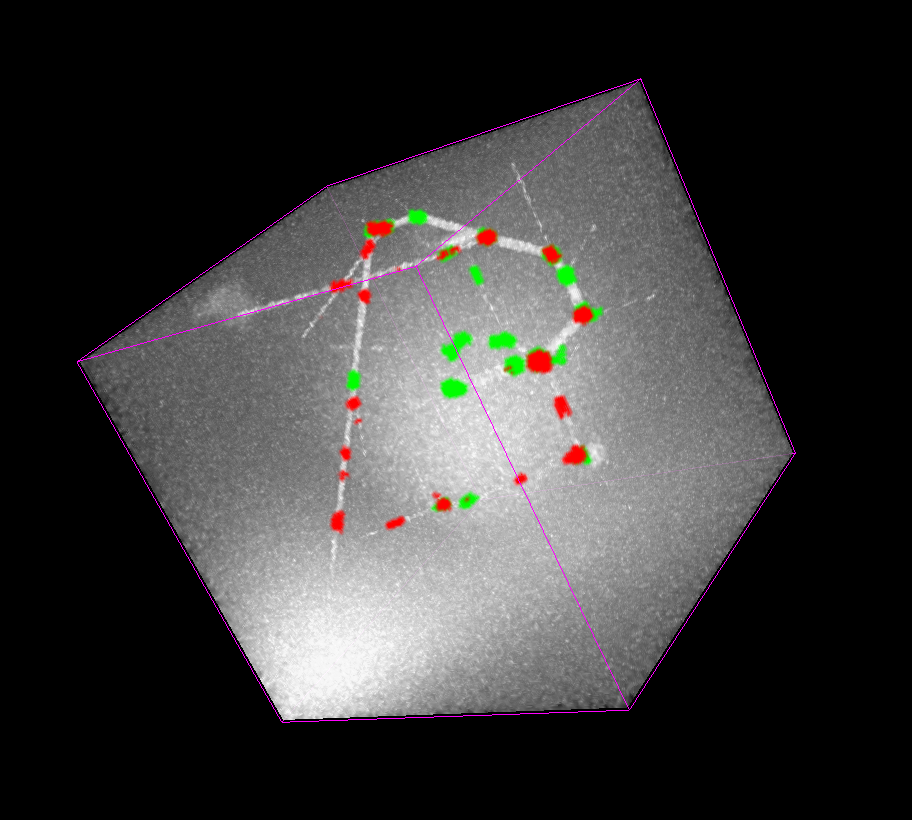
\includegraphics[width=\textwidth]{Images/exp_seg_200.png}
        \caption{Itération 200}
    \end{subfigure}
    \caption{Phases d'entrainement de Unet pour la segmentation des bifurcations. Inférence à l'itération 40, 100 et 200 de l'entrainement. Volume en gris, vérités terrain des bifurcations en vert et sortie du réseau en rouge. }
    \label{fig:seg_deep}
\end{figure}

Afin de contourner ces problèmes, nous avons changé d'objectif en nous concentrant sur la classification de patchs d'images de bifurcations. Dans cette expérience, l'objectif était d'apprendre à un réseau à identifier si un patch contenait une bifurcation centrée sur celui-ci ou non. Lors de la génération des vaisseaux des jeux de données VascuSynth, un fichier contenant les positions des bifurcations est généré. La position des bifurcations est donc connue par construction.

Dans ce nouveau contexte, la tâche à effectuer par le réseau passe d'une segmentation voxélique à une classification binaire des patchs. Nous avons donc remplacé le réseau Unet par un réseau de classification inspiré de l'architecture VGG. Cette architecture se présente sous la forme d'un encodeur formé de couches convolutionnelles suivies de couches de neurones entièrement connectées. La sortie du réseau est formée d'un seul neurone donnant la probabilité d'appartenance d'un patch à une bifurcation. 

Afin de limiter le nombre de bifurcations par patch, nous avons défini une taille de patch de $16 \times 16 \times 16$. Cette taille limite cependant la profondeur du réseau dont certaines opérations réduisent la taille spatiale du volume d'entrée.

\begin{figure}[!ht]
    \centering
    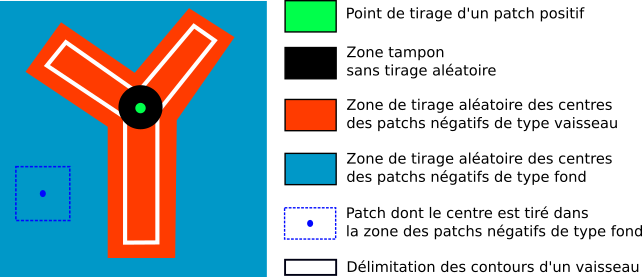
\includegraphics[width=\textwidth]{Images/drawing_patch_area.png}
    \caption{Illustration des zones dans lesquelles sont tirés les patchs. Les patchs négatifs sont tirés parmi deux zones : le voisinage des vaisseaux (rouge) et le fond (bleu). Ces zones permettent d'assurer la présence de vaisseaux parmi les patchs négatifs.}
    \label{fig:drawing_patch_area}
\end{figure}

Il a ensuite été nécessaire de construire un jeu de données de patchs contenant un ensemble représentatif de toutes structures présentes dans les images. Nous avons donc dû nous assurer que des bifurcations, des vaisseaux et des éléments constituant le fond étaient présents dans le jeu de données. Les patchs positifs, ont été simples à construire, car ils regroupent tous les patchs dont le centre est positionné au niveau des coordonnées des bifurcations. Les patchs négatifs ont nécessité plus d'attention, car les vaisseaux ne représentent que $5\percent{}$ des volumes. Un tirage aléatoire des patchs de fond dans les images ne permet donc pas de s'assurer que des patchs contenant des vaisseaux soient présents dans le jeu de données. Les patchs sont alors tirés de manière semi-aléatoire dans deux zones distinctes : le voisinage des vaisseaux et la zone hors de ce voisinage. Dans la zone du voisinage des vaisseaux, on retire une zone de rayon $8$ voxels au niveau des bifurcations de manière à éviter les patchs proches des bifurcations. Les différentes zones sont illustrées dans la figure \ref{fig:drawing_patch_area}.


\begin{figure}[!ht]
    \centering
    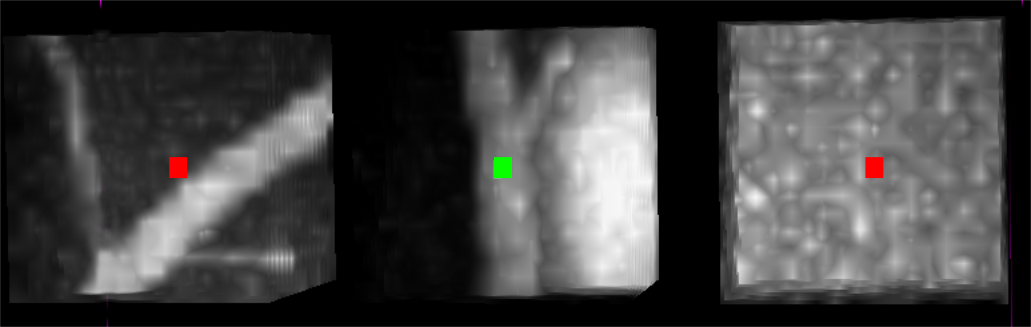
\includegraphics[height=4cm]{Images/exp_patchs_exemple.png}
    \caption{Trois exemples de patchs ; de gauche à droite : patch négatif contenant des vaisseaux, patch positif centré sur une bifurcation et patch négatif de bruit. Les patchs négatifs qui contiennent des vaisseaux peuvent parfois contenir des bifurcations adjacentes non centrées.}
    \label{fig:exp_patchs}
\end{figure}

Dans un premier temps, nous n'avons pas réussi à faire converger notre réseau, malgré de multiples tentatives et de variations du jeu de données et de la configuration du réseau. Nous avons notamment fait varier la proportion et la quantité de patchs de bifurcations dans le jeu de données. Nous avons aussi fait varier le nombre de couches du réseau ainsi que le taux d'apprentissage, l'utilisation des couches de pooling et la fonction de coût sans succès. Nous sommes ensuite parvenus à faire converger le réseau en augmentant la taille des patchs de  $16 \times 16 \times 16$ à $32 \times 32 \times 32$.

Les résultats de classification des patchs ont été encourageants, avec une bonne détection des patchs des bifurcations pour ce jeu de données. Nous avons alors tenté d'appliquer la classification sur l'ensemble d'un volume témoin grâce à un mécanisme de fenêtre glissante. Nous avons alors observé que le réseau identifiait le centre des vaisseaux comme appartenant à une bifurcation. Ce comportement est intéressant, car il révèle une faiblesse de notre méthode (Fig. \ref{fig:exp_patchs}). En effet, nous avons tiré une partie des patchs négatifs dont le centre est aléatoirement distribué dans le voisinage des vaisseaux. Il y a donc une faible probabilité que des patchs négatifs soient centrés sur la ligne centrale des vaisseaux (Fig. \ref{fig:exp_patchs} (a)). Or, toutes nos bifurcations labellisées positives sont localisées le long de la ligne centrale des vaisseaux. Dans le cas où le réseau identifie les voxels le long de la ligne centrale comme des bifurcations, notre jeu de données ne permet pas de différencier les voxels de ligne centrale des voxels de bifurcations (Fig. \ref{fig:inference_patches_vs_sliding_window}).

\begin{figure}[!ht]
    \centering
    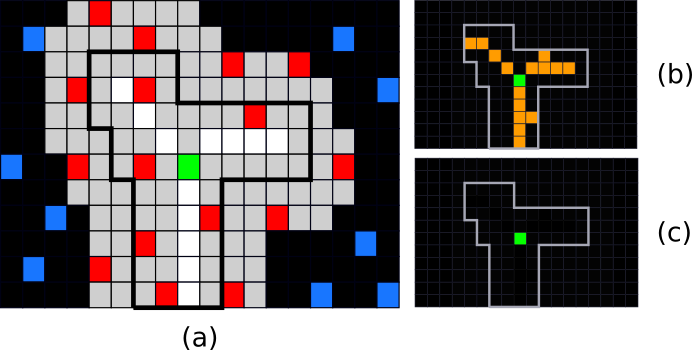
\includegraphics[width=\textwidth]{Images/exp_biais.png}
    \caption{Illustration de la problématique du tirage aléatoire de la position des patchs pour la détection de bifurcations. (a) Le tirage de patchs de bifurcation (vert), négatifs avec vaisseaux (rouges) et négatifs sans vaisseaux (bleu) a peu de chances d'être effectué sur la ligne centrale des vaisseaux. Un réseau entrainé sur une base de données centréés de cette manière peut apprendre la configuration (b) et obtenir de bonnes performances de classification alors que la configuration (c) est attendue.}
    \label{fig:exp_patchs}
\end{figure}

De plus, les zones que nous avons définies pour le tirage aléatoire des centres des patchs dépend des masques de voisinages des vaisseaux, et donc des vérités terrains voxéliques des vaisseaux. Cependant, ces masques vont à l'encontre des contraintes d'annotations que nous nous sommes fixées puisque les annotations des bifurcations ne suffisent pas dans ce cas de figure.

Nous avons dû trouver une méthode de tirage qui ne nécessitait pas de vérité terrain des vaisseaux et qui favorisait le tirage de patchs le long de la ligne centrale dans le but que le réseau différencie ligne centrale et bifurcations. Nous avons donc procédé au tirage des patchs négatifs contenant des vaisseaux en utilisant la carte de probabilité générée par un filtre de rehaussement, plutôt que d'utiliser une zone binaire. Les patchs dont le centre est proche de la ligne centrale des vaisseaux ont ainsi une probabilité plus élevée d'être tirés que les patchs en périphérie des vaisseaux. De cette manière, nous pensions à la fois nous passer d'annotations des vaisseaux et pousser le réseau à différencier les voxels de bifurcations des voxels de la ligne centrale. Cette méthode n'a cependant pas réglé le problème de l'apprentissage.

\begin{figure}[!ht]
    \captionsetup[subfigure]{justification=centering}
    \centering
    \begin{subfigure}{0.48\textwidth}
        \adjincludegraphics[width=\textwidth,trim={{0.15\width} {0\height} {0.1\width} {0.05\height}},clip]{Images/exp_patches_visualization.png}
        \caption{}
    \end{subfigure}
    \begin{subfigure}{0.48\textwidth}
    \adjincludegraphics[width=\textwidth,trim={{0.15\width} {0\height} {0.1\width} {0.05\height}},clip]{Images/exp_sliding_window.png}
    \caption{}
    \end{subfigure}
    \caption{Exemple de résultats de classification sur un échantillon de patchs et sur un volume entier par fenêtre glissante. (a) Chaque point représente le centre d'un patch de taille $32 \times 32 \times 32$ dont le code couleur est le suivant : VP=vert, VN=rouge, FP=jaune, FN=violet. Avec cette représentation, le réseau semble produire une bonne classification. (b) Classification effectuée par fenêtre glissante de l'ensemble des voxels de l'image. La probabilité d'appartenance d'un voxel à une bifurcation est représentée en jaune. Cette visualisation montre que le réseau n'a pas appris à distinguer les bifurcations.}
    \label{fig:inference_patches_vs_sliding_window}
\end{figure}

Ce travail sur la détection des bifurcations pour ensuite segmenter les vaisseaux est un travail préliminaire que nous n'avons pas pu achever. Nous avons toutefois proposé une piste et une méthodologie crédibles qui nécessiteraient d'être poursuivies.

\section{ Bilan des travaux}

Nous avons articulé l'ensemble de nos travaux de manière à ce qu'ils constituent un socle de connaissances et d'outils pour une personne souhaitant approfondir ses connaissances sur les filtres de rehaussement de vaisseaux. 

Nous avons dans un premier temps établi un état de l'art des filtres de rehaussement recouvrant les vingts dernières années. Nous avons ensuite identifié sept filtres représentatifs de la littérature. Nous avons aussi explicité les différents cadres d'espaces d'échelles qui permettent au rehaussement d'être efficace sur l'ensemble du réseau vasculaire malgré des variations de taille importantes des vaisseaux.

Nous avons ensuite décidé d'améliorer l'accessibilité des filtres de rehaussement en proposant de rassembler, adapter et réimplémenter les sept filtres dans un cadre commun en C++. Un utilisateur souhaitant utiliser des filtres de rehaussement, peut ainsi éviter de passer par cette étape très chronophage de recherche et d'adaptation de filtres provenant de sources multiples. 

Puis, nous avons proposé un banc de test, permettant de comparer les performances de ces filtres de manière qualitative et quantitative dans différents contextes. Assez tôt dans sa conception, nous avons fait en sorte que celui-ci soit modulable et extensible par d'autres utilisateurs par l'ajout de nouveaux filtres, zones d'intérêt ou jeux de données. Cet outil permet ainsi de faciliter l'évaluation d'une nouvelle contribution par rapport aux filtres de la littérature.

Les expériences que nous avons menées avec ce banc de test ont mis en valeur des différences significatives entre les filtres de rehaussement. Les filtres hessiens ou de flux proposent des rehaussements lisses, mais parfois surestimés ou rehaussant des bords d'organes. A l'inverse, RORPO est plus précis dans les structures rehaussées, mais leur aspect est beaucoup plus irrégulier. Les filtres se distinguent aussi par leur résistance au bruit avec des filtres plutôt performants pour de faibles niveaux de bruits, comme Jerman et Sato, mais dont les performances chutent lorsque le bruit augmente. À l'inverse le filtre de Frangi propose un mécanisme intéressant pour le contrôle du bruit.

Nous avons aussi fait en sorte que les implémentations des filtres et du banc de test soient à la fois complémentaires et indépendants. De cette manière, chaque partie peut être réutilisée et intégrée séparément selon l'utilisation souhaitée. Nous avons d'ailleurs tiré parti de cette propriété en proposant une démonstration en ligne des filtres qui permet de tester, sans installation, les filtres de rehaussement sur des données de l'utilisateur. L'intégration des filtres de rehaussement a aussi été réalisée dans un logiciel de visualisation d'images médicales : 3DSlicer. Les filtres peuvent ainsi être directement utilisés de manière interactive dans celui-ci.

Enfin, pour compenser le manque d'annotations, nous avons participé à l'élaboration d'un plug-in de segmentation, afin que les bases de données hépatiques avec annotations des vaisseaux se démocratisent. Nous avons aussi exploré une méthode de segmentation à partir des seules annotations des bifurcations.

Nous avons finalement élaboré un travail couvrant tous les aspects nécessaires à l'étude du rehaussement : le développement des bases de données, la théorie du rehaussement, la mise en pratique des filtres ainsi que leur évaluation.